\documentclass[11pt,a4paper]{article}
\usepackage[utf8]{inputenc}
\usepackage[T1]{fontenc}
\usepackage[english]{babel}
\usepackage{lmodern}
\usepackage{amsmath,amssymb}
\usepackage{bm}
\usepackage{booktabs,array}
\usepackage{graphicx}
\usepackage{tikz}
\usepackage[margin=2.5cm]{geometry}
\usepackage{hyperref}

\newcommand{\vm}{\bm{m}}
\newcommand{\vs}{\bm{s}}
\newcommand{\ee}{\mathrm{e}}
\emergencystretch=3em

\title{Spin injection through a polarizer stack:\\
  the one-dimensional Valet--Fert test case}
\author{}
\date{\today}

\begin{document}

\maketitle

\begin{abstract}
  This document comes with the validation case
  \texttt{validation/valet\_fert\_1d} of the branch \texttt{slonczewski}
  of feeLLGood. It explains the Valet--Fert model (two-current model with
  spin diffusion), the assumptions of the test case, the equation solved
  and its analytic solution, how feeLLGood solves the same problem
  (polarizer stack not meshed, Robin condition on the inlet surface), and
  the expected results. The derivations are given in full; a simple result
  comes out of them: the polarization of the injected current is the
  average of the polarizations of the elements of the stack, weighted by
  their spin resistances.
\end{abstract}

\tableofcontents

\section{Purpose of the test}

On the branch \texttt{slonczewski}, the polarized current is no longer
injected with a prescribed polarization. The polarizer F1, the spacer N and
the two interfaces F1/N and N/F2 are not meshed: they are eliminated
analytically and replaced by a Robin condition on the inlet surface of the
sample F2 (key \texttt{slonczewski} of a surface region,
\texttt{src/slonczewskiInterface.h},
\texttt{spinAcc::stackBoundaryCondition}).

The test checks this condition on the simplest case with an exact
solution: a wire, collinear magnetizations, a uniform current. The problem
is then the one solved by Valet and Fert in 1993 for the current
perpendicular to plane giant magnetoresistance (CPP-GMR). In particular,
it checks:
\begin{itemize}
  \item the conversion, done by feeLLGood, of the interface parameters of
    the literature ($AR^*$ in $\Omega\,$m$^2$, asymmetry $\gamma$) into
    conductances of the spin diffusion problem;
  \item the renormalization by the bulk of F1 (finite thickness, reservoir
    on its far side);
  \item the elimination of the spacer node;
  \item the equivalence between the bulk equations of feeLLGood
    (anisotropic diffusion of Zhang--Levy--Fert with $\beta=\beta'=P$) and
    those of Valet--Fert.
\end{itemize}
The transverse terms (mixing conductance $G_{\uparrow\downarrow}$, s--d
precession) play no role here: they are validated by the case
\texttt{validation/slonczewski\_angle}.

\section{The Valet--Fert model}

\subsection{Assumptions}

\begin{enumerate}
  \item \textbf{Diffusive regime.} The mean free path $\lambda$ is small
    compared to the spin diffusion length $l_{sf}$: the Boltzmann equation
    can be replaced by drift--diffusion equations for electrochemical
    potentials. Valet and Fert showed that this is the exact limit of the
    Boltzmann equation when $\lambda\ll l_{sf}$.
  \item \textbf{Two currents.} The electrons of majority moment ($+$,
    moment parallel to the magnetization) and minority moment ($-$)
    conduct in parallel, with their own conductivities $\sigma_\pm$ and
    electrochemical potentials $\mu_\pm$. They mix only by spin flip,
    slower than the other collisions.
  \item \textbf{Collinearity.} All magnetizations are parallel or
    antiparallel to a single axis $z$. The spin accumulation is then a
    scalar (its component along $z$) and the mixing conductances do not
    enter.
  \item \textbf{Linear response, steady state.} The deviations from
    equilibrium are proportional to the current; the steady state is
    sought.
  \item \textbf{One dimension.} The current is uniform and perpendicular to
    the layers; everything depends on the single coordinate $x$ along the
    stack.
  \item \textbf{Thin interfaces.} An interface is a layer of zero thickness
    that conserves spin, characterized by spin-dependent resistances per
    unit area, $r_\pm = 2AR^*(1\mp\gamma)$. There is no spin memory loss
    at the interface.
  \item \textbf{Reservoirs.} Far from the stack (contacts), the electrons
    are at equilibrium: the spin accumulation vanishes there.
\end{enumerate}

\subsection{Two-current Ohm's law}

Here $e>0$ (elementary charge). For each channel, the charge current
density $j_\pm$ obeys the generalized Ohm's law
\begin{equation}
  j_\pm = \frac{\sigma_\pm}{e}\,\frac{d\mu_\pm}{dx},
  \qquad
  \sigma_\pm = \frac{\sigma}{2}\,(1\pm\beta),
  \label{eq:ohm}
\end{equation}
where $\sigma$ is the total conductivity and $\beta$ the bulk
polarization, $0\le\beta<1$ ($\beta = P$ in feeLLGood). The electrons go
down the gradient of $\mu_\pm$; the charge current, of opposite direction,
goes up. We introduce the mean potential and the spin accumulation,
expressed in volts:
\begin{equation}
  \bar\mu = \frac{\mu_++\mu_-}{2},
  \qquad
  \varphi = \frac{\mu_+-\mu_-}{2e},
  \qquad
  \mu_\pm = \bar\mu \pm e\varphi .
\end{equation}
The total current $j = j_++j_-$ and the spin current $j_s = j_+-j_-$
(expressed as a charge current) are
\begin{equation}
  j = \frac{\sigma}{e}\,\bar\mu' + \sigma\beta\,\varphi',
  \qquad
  j_s = \frac{\sigma\beta}{e}\,\bar\mu' + \sigma\,\varphi' .
\end{equation}
Eliminating $\bar\mu'$ between both:
\begin{equation}
  \boxed{\;j_s = \beta\,j + \sigma(1-\beta^2)\,\varphi'\;}
  \label{eq:js-volume}
\end{equation}
The first term is the \emph{drift} spin current: far from any interface, a
fraction $\beta$ of the current is polarized. The second one is a
diffusion current, with the spin conductivity $\sigma(1-\beta^2) =
1/\rho^*$ (notation of Valet--Fert, $\rho^* = \rho/(1-\beta^2)$).

\subsection{Diffusion equation}

Charge is conserved, $j' = 0$: $j$ is uniform. Spin is not: spin flips
relax $\varphi$, and
\begin{equation}
  j_s' = \frac{\sigma(1-\beta^2)}{l_{sf}^2}\,\varphi .
\end{equation}
This relation defines the spin diffusion length $l_{sf}$ (written
$l_{sf}^*$ by Baltz).
With \eqref{eq:js-volume} and $j' = 0$, it gives the Valet--Fert equation:
\begin{equation}
  \boxed{\;\varphi'' = \frac{\varphi}{l_{sf}^2}\;}
  \label{eq:diffusion}
\end{equation}
In each layer, $\varphi$ is a combination of $\ee^{x/l_{sf}}$ and
$\ee^{-x/l_{sf}}$: the spin accumulation is created at the interfaces and
decays over $l_{sf}$ on both sides.

\paragraph{Remark: $l_{sf}$ and the lengths per channel.} Valet and Fert
write $1/l_{sf}^2 = 1/l_{sf,+}^2 + 1/l_{sf,-}^2$, where
$l_{sf,\pm} = \sqrt{D_\pm\tau_\pm}$ involves the time $\tau_\pm$ after which
\emph{one} electron of the channel $\pm$ flips its spin. There is no
factor 2: the difference $\mu_+-\mu_-$ decreases both when a $+$ becomes a
$-$ and when a $-$ becomes a $+$, and the two rates add up like
conductances in parallel. In a normal metal, $l_{sf,+} = l_{sf,-} = l_0$
gives $l_{sf} = l_0/\sqrt2$: the accumulation relaxes twice as fast as a
single electron flips its spin. $l_{sf}$ is thus not an average of the
$l_{sf,\pm}$; it is smaller than each of them. It is the only measurable
length (decay length of $\varphi$, obtained for instance from the CPP-GMR),
and it is the one feeLLGood takes as a parameter (\texttt{l\_sf}); the
$l_{sf,\pm}$ do not enter.

\subsection{Interface conditions}

At an interface of resistances $r_\pm = 2AR^*(1\mp\gamma)$, each channel
goes through a resistance, and $\mu_\pm$ jumps:
$j_\pm = \Delta\mu_\pm/(e\,r_\pm)$, with $\Delta\mu_\pm = \Delta\bar\mu \pm
e\,\Delta\varphi$ (jump right minus left). With
$1/r_\pm = (1\pm\gamma)/\left(2AR^*(1-\gamma^2)\right)$:
\begin{equation}
  j = \frac{\Delta\bar\mu/e + \gamma\,\Delta\varphi}{AR^*(1-\gamma^2)},
  \qquad
  j_s = \frac{\gamma\,\Delta\bar\mu/e + \Delta\varphi}{AR^*(1-\gamma^2)} .
\end{equation}
Eliminating $\Delta\bar\mu$ gives the interface law, of the same form as
\eqref{eq:js-volume}:
\begin{equation}
  \boxed{\;j_s = \gamma\,j + \frac{\Delta\varphi}{AR^*}\;}
  \label{eq:js-interface}
\end{equation}
$\gamma$ plays for the interface the role of $\beta$ for the bulk, and
$AR^*$ the role of the spin resistance. The currents $j$ and $j_s$ are
continuous through the interface (no spin loss).

\subsection{A common frame: the spin resistance}

Relations \eqref{eq:js-volume} and \eqref{eq:js-interface} have the same
structure. For an element $k$ of the stack (bulk or interface), the spin
current through it reads
\begin{equation}
  j_s = P_k\,j + \frac{\Delta\varphi_k}{r_k},
  \label{eq:element}
\end{equation}
where $P_k$ is its polarization, $r_k$ its spin resistance (in
$\Omega\,$m$^2$) and $\Delta\varphi_k$ the variation of $\varphi$ through
it (right minus left). It is a Norton generator: a current source $P_kj$
in parallel with a resistance $r_k$. The bulk layers reduce to it when the
spin current is conserved at their boundary, which is the case of both
layers of the test (section~\ref{sec:circuit}).

\section{The test case}

\subsection{Geometry}

\begin{figure}[h]
\centering
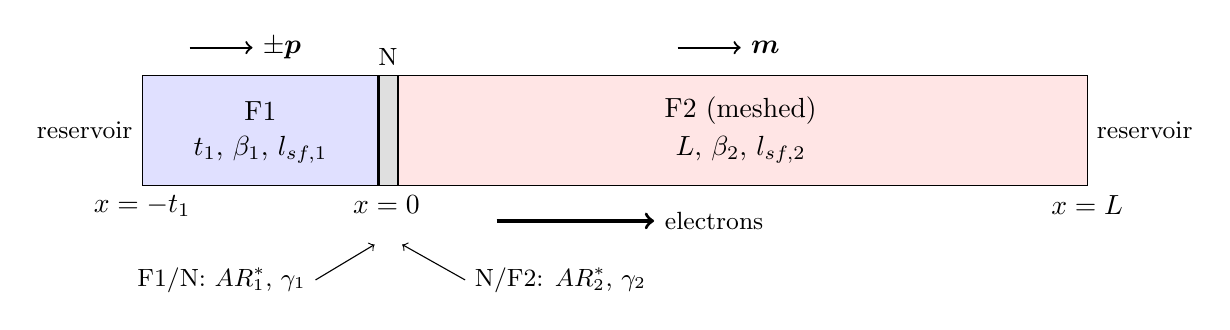
\begin{tikzpicture}[x=1cm,y=1cm]
  \fill[blue!12] (0,0) rectangle (3,1.4);
  \fill[gray!25] (3,0) rectangle (3.25,1.4);
  \fill[red!10] (3.25,0) rectangle (12,1.4);
  \draw (0,0) rectangle (12,1.4);
  \draw[thick] (3,0) -- (3,1.4);
  \draw[thick] (3.25,0) -- (3.25,1.4);
  \node at (1.5,0.95) {F1};
  \node at (1.5,0.45) {$t_1$, $\beta_1$, $l_{sf,1}$};
  \node at (7.6,0.95) {F2 (meshed)};
  \node at (7.6,0.45) {$L$, $\beta_2$, $l_{sf,2}$};
  \draw[->,thick] (0.6,1.75) -- (1.4,1.75) node[right] {$\pm\bm{p}$};
  \draw[->,thick] (6.8,1.75) -- (7.6,1.75) node[right] {$\vm$};
  \node[below] at (0,0) {$x=-t_1$};
  \node[below] at (3.1,0) {$x=0$};
  \node[below] at (12,0) {$x=L$};
  \node[above] at (3.12,1.4) {\small N};
  \draw[<-] (2.95,-0.75) -- (2.2,-1.2) node[left] {\small F1/N: $AR_1^*$, $\gamma_1$};
  \draw[<-] (3.3,-0.75) -- (4.1,-1.2) node[right] {\small N/F2: $AR_2^*$, $\gamma_2$};
  \node[left] at (0,0.7) {\small reservoir};
  \node[right] at (12,0.7) {\small reservoir};
  \draw[->,very thick] (4.5,-0.45) -- (6.5,-0.45) node[right] {\small electrons};
\end{tikzpicture}
\caption{The stack. Only F2 is meshed; F1, the spacer N (of zero
  thickness) and both interfaces are eliminated analytically. The
  electrons flow from F1 to F2.}
\label{fig:stack}
\end{figure}

The stack is shown in figure~\ref{fig:stack}. The axis $x$ of the model is
the axis $z$ of the mesh. The sample F2 is a wire of cross-section
$10\times10$\,nm$^2$ and length $L = 300$\,nm (\texttt{wire.geo}, mesh size
$h = 1$\,nm, 30\,607 nodes, P1 tetrahedra). Its side faces let through
neither charge nor spin (zero Neumann condition): the problem stays
one-dimensional. The magnetizations are along $z$: F2 along $+z$, F1
along $+z$ (configuration P) or $-z$ (AP). In AP, $\beta_1$ and $\gamma_1$
change sign.

\subsection{Parameters}

\begin{center}
\renewcommand{\arraystretch}{1.2}
\begin{tabular}{llll}
  \toprule
  Element & Parameter & Value & feeLLGood key \\
  \midrule
  F2 (wire) & $\sigma_2$ & $4\times10^6$\,S/m & \texttt{sigma} \\
    & $\beta_2$ & 0.3 & \texttt{P} \\
    & $l_{sf,2}$ & 10\,nm & \texttt{l\_sf} \\
    & $l_{sd}$ & 1\,nm & \texttt{l\_sd} \\
    & $N_0$ & $1.344\times10^{47}$\,J$^{-1}$m$^{-3}$ & \texttt{dens\_state} \\
  F1 & $\sigma_1$ & $2\times10^6$\,S/m & \texttt{F1.sigma} \\
    & $\beta_1$ & 0.5 & \texttt{F1.P} \\
    & $l_{sf,1}$ & 20\,nm & \texttt{F1.l\_sf} \\
    & $t_1$ & 15\,nm & \texttt{F1.thickness} \\
  F1/N & $AR_1^*$, $\gamma_1$ & $0.5\times10^{-15}\,\Omega\,$m$^2$, 0.75
    & \texttt{F1N.AR}, \texttt{F1N.gamma} \\
  N/F2 & $AR_2^*$, $\gamma_2$ & $0.3\times10^{-15}\,\Omega\,$m$^2$, 0.6
    & \texttt{NF2.AR}, \texttt{NF2.gamma} \\
  Current & $j_n$ & $10^{12}$\,A/m$^2$ & \texttt{jn} (inlet) \\
  \bottomrule
\end{tabular}
\end{center}

The outward normal of the inlet surface is $-z$; $j_n = \bm{J}\cdot\bm{n}
> 0$ means that the charge current leaves F2 through the inlet, so that
the electrons enter it. The charge current along $x$ is $j = -j_n$. The
mixing conductances (\texttt{Gr} $= 5\times10^{14}$\,S/m$^2$) are given
but do not enter.

\subsection{Boundary conditions}

\begin{itemize}
  \item $x = -t_1$ (reservoir behind F1): $\varphi = 0$;
  \item $x = L$ (outlet, reservoir): $\varphi = 0$ and $V = 0$
    (\texttt{outlet}: \texttt{V: 0}, \texttt{s: [0,0,0]});
  \item $x = 0$: interfaces F1/N and N/F2 on both sides of N, with
    \eqref{eq:js-interface}, and continuity of $j_s$ through N.
\end{itemize}

\section{Analytic solution}

\subsection{The linear system}

We write, with $\ee_1 = \ee^{-t_1/l_{sf,1}}$ and $\ee_2 = \ee^{-L/l_{sf,2}}$,
\begin{align}
  \varphi_1(x) &= a_1\,\ee^{x/l_{sf,1}} + d_1\,\ee^{-(x+t_1)/l_{sf,1}},
    & -t_1 &\le x\le 0, \\
  \varphi_2(x) &= a_2\,\ee^{-x/l_{sf,2}} + d_2\,\ee^{(x-L)/l_{sf,2}},
    & 0 &\le x\le L,
\end{align}
and $\varphi_N$ the accumulation in the spacer. The five unknowns
$(a_1, d_1, \varphi_N, a_2, d_2)$ are given by:
\begin{enumerate}
  \item $\varphi_1(-t_1) = 0$;
  \item $\varphi_2(L) = 0$;
  \item the spin current leaving F1 at $x=0^-$, given by
    \eqref{eq:js-volume}, is the one of the interface F1/N:
    $\beta_1 j + c_1\varphi_1'(0) = \gamma_1 j + (\varphi_N-\varphi_1(0))/AR_1^*$;
  \item it goes through the spacer:
    $\gamma_1 j + (\varphi_N-\varphi_1(0))/AR_1^* =
     \gamma_2 j + (\varphi_2(0)-\varphi_N)/AR_2^*$;
  \item it enters F2:
    $\gamma_2 j + (\varphi_2(0)-\varphi_N)/AR_2^* = \beta_2 j + c_2\varphi_2'(0)$,
\end{enumerate}
with $c_k = \sigma_k(1-\beta_k^2)$. This is the $5\times5$ system solved by
the function \texttt{valet\_fert} of the script. The spin accumulation of
feeLLGood follows (section~\ref{sec:conversion}):
$s_z(x) = \mu_B N_0\,e\,\varphi_2(x)/2$.

\subsection{Circuit reading: the injected polarization}
\label{sec:circuit}

The system can also be solved by hand, and the solution has a simple
interpretation. Since $L = 30\,l_{sf,2}$, F2 can be taken semi-infinite
($\ee_2 \simeq 10^{-13}$): $\varphi_2(x) = \varphi_2(0)\,\ee^{-x/l_{sf,2}}$,
hence $\varphi_2'(0) = -\varphi_2(0)/l_{sf,2}$ and
\begin{equation}
  j_s(0^+) = \beta_2\,j + \frac{0-\varphi_2(0)}{r_2},
  \qquad r_2 = \frac{l_{sf,2}}{\sigma_2(1-\beta_2^2)} = \rho_2^*\,l_{sf,2} .
\end{equation}
F2 is the element \eqref{eq:element} of polarization $\beta_2$ and spin
resistance $r_2$, $\varphi$ going from $\varphi_2(0)$ to 0 far away.
Likewise, in F1, $\varphi_1(x) = \varphi_1(0)\sinh\left((x+t_1)/l_{sf,1}\right)/
\sinh(t_1/l_{sf,1})$, hence
\begin{equation}
  j_s(0^-) = \beta_1\,j + \frac{\varphi_1(0)-0}{R_1},
  \qquad R_1 = \rho_1^*\,l_{sf,1}\tanh\frac{t_1}{l_{sf,1}} .
\end{equation}
The spin resistance of a layer of finite thickness on a reservoir is
reduced by $\tanh(t_1/l_{sf,1})$: it is the inverse of the conductance
$g_F$ of the note \texttt{slonczewski\_polarisation.tex}.

The spin current $j_s$ is the same in the four elements (F1, F1/N, N/F2,
F2), and the variations of $\varphi$ add up from 0 (reservoir of F1) to 0
(far in F2). Summing \eqref{eq:element},
$\sum_k (j_s - P_kj)\,r_k = 0$, hence
\begin{equation}
  \boxed{\;\frac{j_s}{j} = P_{\mathrm{inj}}
  = \frac{\beta_1R_1 + \gamma_1AR_1^* + \gamma_2AR_2^* + \beta_2r_2}
         {R_1 + AR_1^* + AR_2^* + r_2}\;}
  \label{eq:Pinj}
\end{equation}
\textbf{The polarization of the injected current is the average of the
polarizations of the elements, weighted by their spin resistances.} An
element of large spin resistance imposes its polarization; this is the
origin of the conductivity mismatch (a layer of huge spin resistance, like
a semiconductor, imposes $P_{\mathrm{inj}}\simeq0$).

The accumulation at the inlet of F2 follows:
\begin{equation}
  \boxed{\;\varphi_2(0) = (P_{\mathrm{inj}}-\beta_2)\,j_n\,r_2\;}
  \label{eq:phi0}
\end{equation}
(with $j = -j_n$). The sign of $s$ at the inlet tells whether F2 receives
more majority spin than it can carry in its bulk ($P_{\mathrm{inj}} >
\beta_2$, $s>0$) or less ($s<0$).

\subsection{Numerical values}

The spin resistances are
\begin{center}
\begin{tabular}{lcc}
  \toprule
  Element & $r_k$ ($10^{-15}\,\Omega\,$m$^2$) & $P_k$ (P / AP) \\
  \midrule
  F1, $R_1 = \rho_1^*l_{sf,1}\tanh(t_1/l_{sf,1})$ & 8.469 & $+0.5$ / $-0.5$ \\
  F1/N, $AR_1^*$ & 0.5 & $+0.75$ / $-0.75$ \\
  N/F2, $AR_2^*$ & 0.3 & 0.6 \\
  F2, $r_2 = \rho_2^*l_{sf,2}$ & 2.747 & 0.3 \\
  \midrule
  Total & 12.016 & \\
  \bottomrule
\end{tabular}
\end{center}
and \eqref{eq:Pinj} gives
\begin{center}
\renewcommand{\arraystretch}{1.2}
\begin{tabular}{lccc}
  \toprule
  & $P_{\mathrm{inj}}$ & $\varphi_2(0)$ (mV) & $s_z(0)$ (A/m) \\
  \midrule
  P  & $+0.467$ & $+0.459$ & $+45.86$ \\
  AP & $-0.300$ & $-1.648$ & $-164.60$ \\
  \bottomrule
\end{tabular}
\end{center}
The ratio AP/P is $(-0.300-0.3)/(0.467-0.3) = -3.59$. These values are
those of the exact solution of the $5\times5$ system (the deviation due to
the finite length of F2 is of order $\ee^{-30}$).

\textbf{Interpretation.} In P, F1 and the interface F1/N, strongly
polarized, inject a current more polarized ($0.467$) than the one F2
carries in its bulk ($0.3$): majority electrons accumulate at the inlet,
$s>0$. In AP, F1 polarizes the current the other way; despite the
interface N/F2 and F2, which pull towards $+0.6$ and $+0.3$, the injected
current is polarized at $-0.30$. The deviation from $\beta_2$ is 3.6 times
larger: minority electrons accumulate, $s<0$, and more strongly. In both
cases, $s$ decays as $\ee^{-x/l_{sf,2}}$: at $x = 10$\,nm, it is $1/\ee$
of its inlet value (16.87\,A/m in P). The difference of the potential
drops between P and AP is the CPP-GMR.

\section{What feeLLGood solves}

\subsection{Bulk equations}
\label{sec:conversion}

feeLLGood solves for the spin accumulation $\vs$ (in A/m)
\begin{equation}
  \nabla\cdot Q = -\frac{\vs}{\tau_{sf}} - \frac{\vs\times\vm}{\tau_{sd}},
  \qquad
  Q_{i\alpha} = -P\,\frac{\mu_B}{e}\,j_i\,m_\alpha
  - D_0\left[\partial_i s_\alpha - P^2 m_\alpha(\vm\cdot\partial_i\vs)\right],
\end{equation}
with $D_0 = 2\sigma/(e^2N_0)$ and, in the magnetic regions,
$1/\tau_{sf} = D_0(1-P^2)/l_{sf}^2$. In the collinear case,
$\vs = s\,\vm$ and $\vs\times\vm = 0$; the diffusion along $\vm$ is
$D_0(1-P^2)$ and the moment flux along $x$ is
\begin{equation}
  Q = -P\,\frac{\mu_B}{e}\,j - D_0(1-P^2)\,s' .
\end{equation}
With $s = \mu_BN_0e\varphi/2$ and $D_0 = 2\sigma/(e^2N_0)$,
$D_0(1-P^2)\,s' = (\mu_B/e)\,\sigma(1-P^2)\,\varphi'$, hence
\begin{equation}
  Q = -\frac{\mu_B}{e}\left[P\,j + \sigma(1-P^2)\,\varphi'\right]
    = -\frac{\mu_B}{e}\,j_s :
\end{equation}
the current of feeLLGood is exactly $-(\mu_B/e)$ times the spin current
\eqref{eq:js-volume} of Valet--Fert, with $\beta = P$. The relaxation
equation likewise gives $s'' = s/l_{sf}^2$, that is \eqref{eq:diffusion}.
The factor $1/2$ of the conversion comes from $D_0$ being twice the
coefficient $D$ of the Einstein relation $\sigma = e^2N_0D$: $\vs$ is half
the physical magnetization $\mu_BN_0\mu_s$, which changes no result.

This equivalence requires the anisotropic diffusion: the key
\texttt{anisotropic\_diffusion} of the section \texttt{spin\_accumulation}
must be \texttt{true}, which is the default. Without it, the spin
conductivity of F2 would be $\sigma$ instead of $\sigma(1-P^2)$ and the test would fail.

\subsection{The Robin condition on the inlet}

The non-meshed stack (F1, F1/N, N, N/F2) is the series connection of the
first three elements of \eqref{eq:element}. Summing their variations of
$\varphi$ between the reservoir of F1 and the inlet of F2:
\begin{equation}
  j_s = P_{\mathrm{st}}\,j + \frac{\varphi_2(0)}{R_{\mathrm{st}}},
  \qquad
  R_{\mathrm{st}} = R_1 + AR_1^* + AR_2^*,
  \qquad
  P_{\mathrm{st}} = \frac{\beta_1R_1 + \gamma_1AR_1^* + \gamma_2AR_2^*}{R_{\mathrm{st}}} .
\end{equation}
Converted into the moment flux entering F2 with $s = \mu_BN_0e\varphi/2$
and $j = -j_n$, this is the Robin condition
\begin{equation}
  \boxed{\;q = \frac{\mu_B}{e}\,j_n\,P_{\mathrm{st}} - G\,s,
  \qquad G = \frac{k}{R_{\mathrm{st}}},\quad k = \frac{2}{e^2N_0}\;}
\end{equation}
($G$ in m/s). This is what feeLLGood builds in the collinear case:
\begin{itemize}
  \item \texttt{Slonczewski::makeStack} converts each interface,
    $G_\parallel = k/AR^*$ and $P = \gamma$;
  \item \texttt{renormalizeF1} puts the bulk of F1,
    $g_F = k/R_1 = k\,\sigma_1(1-\beta_1^2)\coth(t_1/l_{sf,1})/l_{sf,1}$,
    in series with the conductance of F1/N:
    $G_{\parallel1}^* = g_FG_{\parallel1}/(g_F+G_{\parallel1})$ and
    $P_1^* = (\beta_1g_F + \gamma_1G_{\parallel1})/(g_F+G_{\parallel1})$;
  \item \texttt{effectiveBC} eliminates the spacer node: the effective
    conductance is the series connection $G_2(G_1+G_2)^{-1}G_1$, the
    effective polarization the corresponding weighted average.
\end{itemize}
All conductances are converted with the density of states $N_0$ of F2,
the volume region bordering the surface: the one of F1 does not enter.

The discrete problem is the spin diffusion problem of feeLLGood on the
wire with this condition on the inlet and $\vs = 0$ on the outlet. Since
the Robin condition is exact for the non-meshed stack, the only error is
the discretization error in F2.

\section{Expected results}

\subsection{Profiles}

\begin{figure}[h]
\centering
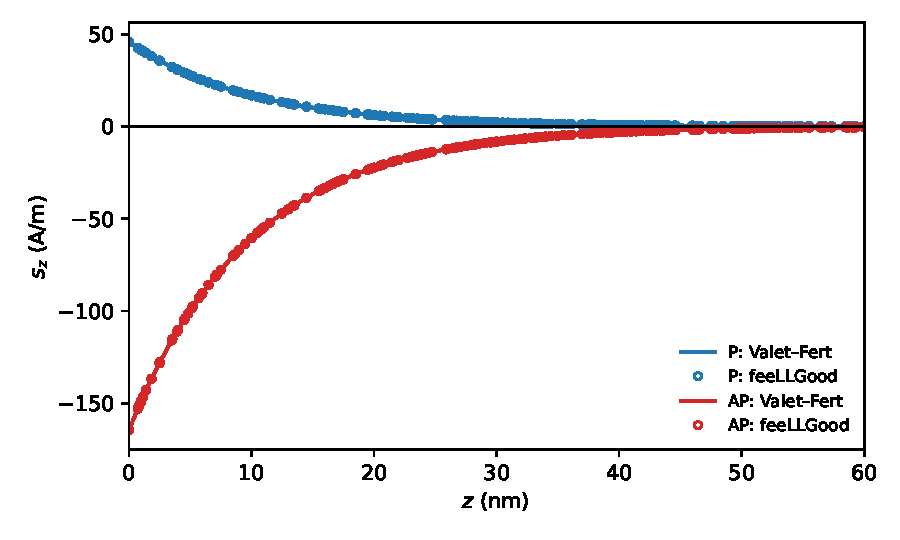
\includegraphics[width=0.8\textwidth]{valet_fert_1d_profile.pdf}
\caption{Spin accumulation $s_z$ along the wire: Valet--Fert solution
  (lines) and feeLLGood values at 250 randomly chosen nodes (circles),
  configurations P and AP, $h = 1$\,nm. Only the first 60\,nm are shown;
  beyond, $s_z$ vanishes.}
\label{fig:profile}
\end{figure}

Figure~\ref{fig:profile} compares both solutions. The nodes at the same
abscissa have the same value to the accuracy of the plot: the solution is
indeed one-dimensional, and its transverse components $s_x$, $s_y$ vanish
(they are exactly 0 in the \texttt{.sol} files).

\subsection{Accuracy and convergence}

The script compares $s_z$ at the nodes to the analytic solution and
computes the maximum error relative to $\max|s_z|$:
\begin{center}
\renewcommand{\arraystretch}{1.2}
\begin{tabular}{lccc}
  \toprule
  Mesh & P: $s_z(0)$ feeLLGood / VF & AP: $s_z(0)$ feeLLGood / VF
    & max error \\
  \midrule
  $h = 2$\,nm & 45.690 / 45.858\,A/m & $-163.994$ / $-164.596$\,A/m
    & $8.2\times10^{-3}$ \\
  $h = 1$\,nm & 45.811 / 45.858\,A/m & $-164.427$ / $-164.596$\,A/m
    & $2.6\times10^{-3}$ \\
  \bottomrule
\end{tabular}
\end{center}
The error decreases as $h^2$, as expected from P1 elements for a smooth
solution. It is the same in P and AP: relative to $\max|s_z|$, it depends
only on the ratio $h/l_{sf,2}$ (here $1/10$) and on the Robin condition,
which has the same form in both cases. The computation takes about 25\,s
for both configurations.

\subsection{What the test detects}

\begin{itemize}
  \item \textbf{Conversion factor.} With $G_\parallel = 1/(e^2N_0AR^*)$
    instead of $2/(e^2N_0AR^*)$, the error rises to 8.5\,\% in P: the test
    fails (tolerance 1\,\%).
  \item \textbf{Renormalization by F1.} Forgetting the bulk of F1
    ($R_1 = 0$) changes $P_{\mathrm{inj}}$ from 0.467 to 0.389 in P
    (formula~\eqref{eq:Pinj}): by \eqref{eq:phi0}, $s_z(0)$ is almost
    halved.
  \item \textbf{Isotropic diffusion.} With
    \texttt{anisotropic\_\allowbreak diffusion: false}, F2 no longer has the
    Valet--Fert equations: the error rises to 7.3\,\% in P and the test
    fails.
\end{itemize}

\subsection{Usage}

\begin{verbatim}
cd validation/valet_fert_1d
./valet_fert.py [path to feellgood]     # default: ../../src/feellgood
\end{verbatim}
The mesh is built with \texttt{gmsh} if missing. The script writes the
settings of each configuration, runs feeLLGood over a very short time (the
spin diffusion problem is stationary and solved at each step), reads the
files \texttt{P\_iter0.sol} and \texttt{AP\_iter0.sol}, and prints:
\begin{verbatim}
P : s_z(inlet) feeLLGood =    45.811 A/m, Valet-Fert =    45.858 A/m;
    max error / max|s| = 2.63e-03, transverse = 0.0e+00
AP: s_z(inlet) feeLLGood =  -164.427 A/m, Valet-Fert =  -164.596 A/m;
    max error / max|s| = 2.63e-03, transverse = 0.0e+00
OK
\end{verbatim}
The exit status is 0 if the error is below 1\,\% in both configurations.

\section{Limitations of the test}

\begin{itemize}
  \item The test is collinear: it says nothing about the mixing
    conductances, the s--d precession, or the choice \texttt{sink} or
    \texttt{series} for the transverse part. The case
    \texttt{validation/slonczewski\_angle} covers them.
  \item F2 is a single region: the continuity of $\vs$ between two meshed
    regions of different densities of states is tested by
    \texttt{validation/two\_regions\_1d}.
  \item The Valet--Fert model has no spin memory loss at the interfaces;
    neither has feeLLGood.
  \item The mesh resolves $l_{sf,2} = 10$\,nm by far. In an actual
    computation, the transverse length $l_{sd}\sim1$\,nm must be resolved
    too, which this test does not check.
\end{itemize}

\section*{References}

\begin{itemize}
  \item T.~Valet, A.~Fert, \emph{Theory of the perpendicular
    magnetoresistance in magnetic multilayers}, Phys.\ Rev.\ B
    \textbf{48}, 7099 (1993).
  \item S.~Zhang, P.\,M.~Levy, A.~Fert, Phys.\ Rev.\ Lett.\ \textbf{88},
    236601 (2002): non-collinear spin diffusion.
  \item A.~Fert, H.~Jaffrès, Phys.\ Rev.\ B \textbf{64}, 184420 (2001):
    spin injection and conductivity mismatch.
  \item V.~Baltz, \emph{The Basics of Electron Transport in Spintronics},
    EDP Sciences (2023), §3.2--3.4 and exercise 6.3.
  \item \texttt{dev-notes/slonczewski\_polarisation.tex} (in French):
    derivation of the Robin condition, renormalization by F1, conversion
    of the conductances.
  \item \texttt{dev-notes/spin\_injection\_boundary\_conditions.md}: the
    same, in English, with the implementation in feeLLGood.
\end{itemize}

\end{document}
